%!TEX root = ../main.tex

\chapter{Introduction} \label{ch:Intro}
Air traffic has increased rapidly over the last five decades, leading to a global increase in emissions of CO$_2$ and other greenhouse gases. This increase can be locally retarded by replacing old aircraft with newer ones \cite{emission}, but this effect is unlikely to be sustained because all forecasts anticipate further rapid increases in air traffic over the coming years \cite{airbus,jadc}. To make flight more sustainable over a longer period of time, continuous performance improvements are needed. Increasing the efficiency of aircraft engines will therefore be a very important element of efforts to improve the emissions performance of air traffic.

Significant improvements in engine efficiency have been achieved in recent decades, especially due to the widespread use of Computational Fluid Dynamics (CFD) simulations. This has enabled the development of high bypass ratio turbofan engines with large fans and high pressure-ratio engine cores that combine relatively high efficiencies, high sub-sonic aircraft velocities, and low noise levels. Unfortunately, further efficiency improvements are getting harder to achieve using current methods. In the design process, engine components are usually divided into several modules, each of which is optimized separately using a simplified interaction scheme. Ghisu et al.\cite{IntegrP2} showed that optimizing components in isolation from each other in this way can yield sub-optimal overall engine designs, which may necessitate expensive redesign work late in the design process. The risk of this can be substantially reduced by adopting more integrated design processes in which multiple components are optimized together. Such integrated processes take advantage of the reduced need for simplified or modeled interactions between components, yielding better optimized solutions at an earlier stage\cite{IntegrP1,IntegrP2}.

\section{The aircraft engine}
%\ignore{Citation missing: Boundary condition effects - 1}
%Describe a turbofan engine\\
Modern high bypass-ratio turbo-fan engines such as that depicted in Figure \ref{fig:engine} have six major {\color{red}aerodynamic} components. The fan, which is located at the engine inlet, accelerates the air; a fraction of this air enters the engine core, but most of it is bypassed. The bypassed air is responsible for the majority of the engine's thrust. Newer high bypass-ratio turbo-fan engines typically have a bypass ratio of 8-12. The low pressure and high pressure compressors (LPC and HPC, respectively) are where the first and second stages of compression are performed, respectively. The combustion chamber (CC) is where the fuel is injected into the compressed air and ignited to increase the energy of the fluid. The high pressure turbine (HPT) is where energy is extracted from the core flow to drive the HPC. The final major aerodynamic component is the low pressure turbine (LPT). In a two-spool engine configuration, the LPT drives both the LPC and the fan. In a three-spool configuration, the LPT has two main components, each of which drives a different shaft to establish different rotational speeds for the fan and the LPC. In the two-spool configuration, different rotational speeds are established using a geared shaft.

\begin{figure}[H]
%Turbofan: https://www.aviationcv.com/aviation-blog/2016/worlds-biggest-jet-engine-first-testing
  %Borja had this reference: http://pw.utc.com/
    \centering
  \begin{tikzpicture}
    \node[anchor=south west,inner sep=0] at (0,0) {\includegraphics[width=0.7\linewidth]{Figures/ge9x.jpg}};
    %\draw[help lines,step=.2] (0,0) grid (10,7);
    \node at (1.2,6.8) {\bf{Fan}};
    \draw[-latex,thick] (1.2,6.6)--(1.85,5.1);
    \node at (3.8,6.8) {\bf{LPC}};
    \draw[-latex,thick] (3.8,6.6)--(4.2,4.3);
    \node at (5.8,5.2) {\bf{ICD}};
    \draw[-latex,thick] (5.8,5.0)--(4.75,3.85);
    \node at (6.4,4.6) {\bf{HPC}};
    \draw[-latex,thick] (6.4,4.4)--(6.,3.6);
    \node at (7.2,5.2) {\bf{CC}};
    \draw[-latex,thick] (7.2,5.)--(7,3.8);
    \node at (8.,6) {\bf{HPT}};
    \draw[-latex,thick] (8,5.8)--(7.6,3.8);
    \node at (9.,5.6) {\bf{LPC}};
    \draw[-latex,thick] (9.,5.4)--(8.6,4.4);


  \end{tikzpicture}
  \caption{The two spool GP7000 turbofan engine\cite{GP7000}}\label{fig:engine}
\end{figure}\noindent

The S-shaped intermediate compressor duct (ICD) located between the LPC and HPC is another important engine component but the analysis and improvement of its performance has attracted less interest than that of the components discussed above. The purpose of the ICD is to guide the flow from the larger radius LPC towards the HPC. The LPC tends to have a large hub-to-tip radius to achieve more efficient compression, whereas the HPC has a lower radius to limit tip leakage losses and reduce disk weight. This means that the ICD must force the flow through an S-shaped annular duct over a large radial offset to maximize the engine's efficiency, but must also have a minimal axial length to limit the engine's size and weight. These competing requirements necessitate an aggressive duct design. However, if the forcing is too aggressive, strong adverse pressure gradients may develop, potentially causing the flow to separate at the convex inner wall. Only a few studies have examined the performance of the S-shaped duct. Britchford et al.\cite{Britchford1994} analyzed the flow field of a clean S-shaped duct and concluded that the flow inside such ducts is complex and influenced by their strong curvature and the streamwise pressure gradient, which gives rise to a high risk of separation at the inner wall. In another study, Britchford et al.\cite{Britchford1994b} showed that an upstream rotor can efficiently re-energize the boundary layer at the inner wall and thereby reduce the adverse pressure gradient, resulting in a lower risk of separation. Bailey et al.\cite{Bailey} showed that the pressure losses of a clean S-shaped duct with a well-behaved flow and no separation were comparable to those for a parallel-sided duct despite the strong curvature and pressure gradient effects. These authors also showed that the presence of a strut imposed blockages that increased pressure losses, resulting in the formation of thicker boundary layers at the inner and outer casings. Karakasis et al.\cite{Karakasis2010} compared experimental data on the performance of axisymmetric and non-axisymmetric ducts to results from CFD simulations. The simulations agreed well with the experimental data for the flow close to the inner casing but did not accurately capture the structure at the outer wall. The study also gave a good description of the mechanics in an ICD with a strut and upstream compressor.

Figure \ref{fig:enginezoom} shows a zoomed-in view of the ICD of the engine depicted in Figure \ref{fig:engine}. The rear stages of the upstream LPC and first stages of the downstream HPC can be seen, along with the radial offset between these two components. To analyze the flow physics of the ICD in detail, an experimental rig has been built at GKN Aerospace in Trollh\"{a}ttan. This rig represents a simplified ICD featuring a strut, upstream guide vanes, and a system representing the last rotating blade row (rotor) of the upstream LPC. Figure \ref{fig:schema} illustrates how the test section of the experimental rig is set up. It consists of pre-swirlers (PSW), a bleed pipe, outlet guide vanes (OGV), and struts, all of which bar the PSW are real engine components. The PSW, which is a stationary blade row, is located upstream of the test section to replicate the rotor exit-flow from the rear stage of a real engine compressor. Using stationary blades results in simpler simulations, minimizing computational costs. The bleed pipe represents the passage through which bleed flow is extracted from the main flow to ensure stable compressor operation at partial speed. The OGVs are placed downstream of the bleed pipe to guide the flow correctly into the ICD. They are integrated into the ICD to minimize their length \cite{Walker2011}, which reduces the risk of separation, and are designed to minimize the upstream effects of the strut's potential field. The strut, which has a zero-lift wing profile, is located inside the duct to add mechanical strength and deliver services to the engine core in the form of oil pipes and electrical cables. However, as discussed above, the strut's presence also increases pressure losses and the complexity of the flow structures in the ICD.
%
\begin{figure}[H]
  \centering
  \begin{tikzpicture}
    \node[anchor=south west,inner sep=0] at (0,0) {  \includegraphics[width=0.5\linewidth, trim=19cm 15cm 22cm 9cm, clip]{Figures/ge9x.jpg}};
    \node at (3.2,4.6) {\bf{Strut}};
    \draw[-latex,thick] (3.2,4.4)--(2.8,3.6);
    \node at (1.,3.2) {\bf{OGV}};
    \draw[-latex,thick] (1.,3.4)--(1.6,4.2);
    \node at (5.6,4.2) {\bf{HPC}};
    \draw[-latex,thick] (5.6,4.)--(5.2,2.2);
%    \draw[help lines,step=.2] (0,0) grid (7,5);
  \end{tikzpicture}
\caption{Zoomed-in view of the ICD, including the last stages of the LPC and first stages of the HPC} \label{fig:enginezoom}
\end{figure}

Aircraft engines typically have 8-10 struts, and the number of OGVs is usually an order of magnitude higher than that of struts. To permit the use of the same tangential sector for all domains in CFD simulations without having to include the full cross-section of the duct, the experimental rig was set up with 9 struts and 81 OGV. The same was done for the PSW, which has 45 blades in total.


%% Original sentence:
%% To obtain the same tangential sector for all domains in CFD simulations without having to include the full 360$^{\circ}$, the experimental rig was set up with 9 struts and 81 OGV. The same was done for the PSW, which has 45 blades in total.
%%

 \begin{figure}[h!]
   \centering
%\documentclass[12pt,english]{article}
%\usepackage{fullpage}
%\usepackage[T1]{fontenc} 
%\usepackage{helvet}
%\renewcommand{\familydefault}{\sfdefault}
%\usepackage{babel}
%\usepackage{amsmath}
%\numberwithin{equation}{section}
%\usepackage{hyperref}
%\usepackage{tikz,pgfplots}
%\usepackage{boldline} %To get thicker lines in tables
%\usepackage{float}    %For float on figures for exampel
%\usepackage{graphicx} %Figures
%
%\usepackage{sectsty}
%\allsectionsfont{\centering}
%
%\renewcommand{\thesubsection}{\Roman{subsection}} 
%\renewcommand{\thesubsubsection}{\Alph{subsubsection}} 
%
%\newcommand{\ignore}[1]{}
%
%\begin{document}
%
%\begin{figure}[H]
%  \centering
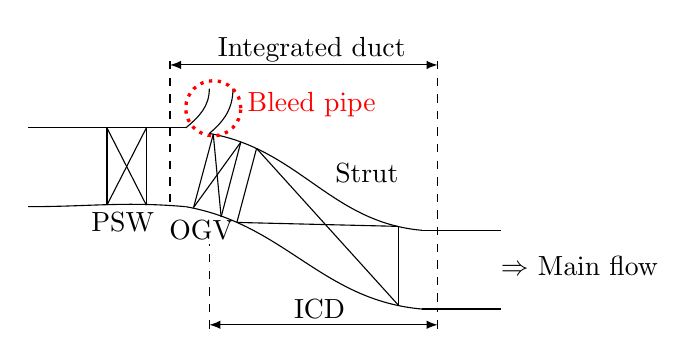
\begin{tikzpicture}
  \coordinate (A) at (-1,1);
  \coordinate (B) at (1,1);
  \coordinate (C) at (1.3,1.5);
  \coordinate (D) at (1.6,1.5);
  \coordinate (E) at (1.3,0.93);
  \coordinate (F) at (4,-0.3);
  \coordinate (G) at (5,-0.3);
  \coordinate (H) at (-1,0);
  \coordinate (I) at (1,0);
  \coordinate (J) at (4,-1.3);
  \coordinate (K) at (5,-1.3);
  %Upper side
  \draw (A)--(B);
  \path [black,out=40,in=-90] (B) edge (C);
  \path [black,out=-90,in=40] (D) edge (E);
  \path [black,out=-10,in=175] (E) edge (F);
  \draw (F)--(G);
  \draw[red,dotted, very thick] (1.35,1.25) circle (0.35);
  \node[red] at ([shift={(1.0,-0.2)}]D) {Bleed pipe};
  %Lower side
  \path [black,out=0,in=175] (H) edge (I);
  \path [black,out=-10,in=175] (I) edge (J);
  \path [black,out=0,in=180] (J) edge (K);
  %PSW
  \draw (0,1)--(0,0.02);
  \draw (0.5,1)--(0.5,0.02);
  \draw (0,0.02)--(0.5,1.0);
  \draw (0.5,0.02) -- (0,1);
  %\node at ([shift={(1.2,0.2)}]A) {PSW};
  %OGV
  \draw (1.35,0.92) -- (1.1,-0.01);
  \draw (1.7,0.82) -- (1.45,-0.13);
  \draw (1.35,0.92) -- (1.45,-0.13);
  \draw (1.7,0.82) -- (1.1,-0.01);
  %\node at ([shift={(0.0,-0.3)}]I) {OGV};
  %Duct
  \draw (1.9,0.74) -- (1.65,-0.2);
  \draw (3.7,-0.25) -- (3.7,-1.25);
  \draw (1.9,0.74) -- (3.7,-1.25);
  \draw (3.7,-0.25) -- (1.65,-0.2);
  %\node at ([shift={(1.8,-0.5)}]E) {Duct};

  %Marking the Integrated duct
  \node at ([shift={(1.0,0.5)}]D) {Integrated duct};
  \draw[latex-latex] (0.8,1.8)--(4.2,1.8);
  \draw[dashed] (0.8,1.85)--(0.8,0);
  \draw[dashed] (4.2,1.85)--(4.2,-1.3);
  %Marking the duct
  \node at ([shift={(-1.3,0.)}]J) {ICD};
  \draw[latex-latex] (1.3,-1.5)--(4.2,-1.5);
  \draw[dashed] (1.3,-1.55)--(1.3,-0.48);
  \draw[dashed] (4.2,-1.55)--(4.2,-1.3);

  %Mark Front Traverse surface
  %\draw[dashed, thick] (0.8,1.2)--(0.8,0);
  %Strut
  \node at ([shift={(2.0,-0.5)}]E) {Strut};
  %PSW
  \node at ([shift={(1.2,-0.2)}]H) {PSW};
  %OGV
  \node at ([shift={(0.2,-0.3)}]I) {OGV};
  %Main flow
  \node at ([shift={(1.0,-0.45)}]G) {$\Rightarrow$ Main flow};
\end{tikzpicture}
%  \caption{Schematic of the integrated compressor duct design}
%  \label{fig:schema}
%\end{figure}
%\end{document}

  \caption{Schematic of the integrated compressor duct design}
  \label{fig:schema}
\end{figure}
%flow field of ICD, Cambridge references. schematic figure\\

There are no practical design rules for ICDs, so their design is usually guided by a combination of CFD and optimization studies. While the ICD has not been optimized to the same extent as the surrounding components, there have been some successful attempts to optimize or analyze its design \cite{CompressorOpt,OptComp1,OptComp2,Walker2011}, resulting in shorter and lighter engines with more aggressive flow guidance. However, the interaction between the duct and the surrounding components has not been addressed in the same way even though it can strongly affect performance \cite{IntegrP2}. If this interaction is neglected, the isolation of the ICD during the design process can limit the design space available for optimization because the duct's internal flow field depends strongly on the surrounding components. Consequently, a more integrated design strategy in which the ICD is introduced earlier in the design process should be considered.

The scope for applying more integrated design strategies is limited to some degree by the availability of computational power because including more components greatly increases computational costs. This is particularly true when dealing with 3D CFD simulations. Furthermore, to take full advantage of CFD simulations and integrated design processes, one must use tools such as the Large Eddy Simulation (LES)model to properly describe flow separation and complicated flow behaviors that are not fully captured by the more common Reynolds Averaged Navier-Stokes (RANS) models. However, LES simulations are very computationally expensive. In an attempt to limit the computational cost of such simulations while still capturing phenomena described poorly by the RANS model, this thesis explores the application of the hybrid LES/RANS Delayed Detached Eddy Simulation (DDES) model introduced by Spalart et al.\cite{DDES}. DDES combines the ability of LES to resolve the transient features of the main flow with the ability of RANS models to model attached near-wall behavior at reasonable grid densities. 

%The original DES model was introduced by Spalart et al\cite{DES97} as a hybrid between LES and RANS turbulence models based on the Spalart-Allmaras (SA) one equation model \cite{SA}. Initially the model was only presented for a 2D application but extended to 3D by Shur et al\cite{DES99}. In that study the performance of the DES model gave a promising result which lead to a wide usage. It was however shown that for grids with stream-wise grid spacings of similar size as the boundary layer a premature switching from RANS to LES could happen. This was the motivation for the new and improved DES, called Delayed DES (DDES)\cite{DDES}. In the DDES model the switching between RANS and LES is no longer governed only by the grid density but also the solution itself. This has greatly improved the application of the model as less time can be spent in generating satisfactory grids. \\
\section{Aim}
The primary objective of the work presented in this thesis was to analyze the flow-physics of the ICD by applying higher fidelity models than have previously been used for this purpose. This was expected to provide new understanding of the complicated flow features present in the duct, particularly those associated with the bleed pipe. Because this proved to be more time-consuming than initially expected due to the challenges of implementing the simulations, simplified modeling techniques were used in these studies. The first step involved applying more common and less computationally demanding models (see Chapter \ref{ch:sim}).

A secondary objective was to evaluate the performance of an in-house code and analyze its application in uncharted areas. This was expected to highlight areas where improvements are needed, leading to the development of a more competitive solver.

%Initial aims:
%Better understanding,
%Expand tools capability,
\chapter{Turbulence modeling}
Turbulence is a three-dimensional, chaotic and unsteady phenomenon governed by the Navier-Stokes equations, which are presented in Chapter \ref{ch:NM}. It controls most flows known in real life situations including the flows around cars, airplanes and trains, as well as high-speed internal flows and flows with geometry-induced turbulence. Its chaotic nature makes it difficult to simulate, typically necessitating at least some use of modeling techniques. 

The Reynolds number, one of the most important quantities in fluid dynamics, is used to distinguish between laminar and turbulent flows. It is defined by Eq. \ref{eq:Re}, and can be interpreted in physical terms as the ratio of the inertial forces to the viscous forces in the fluid under consideration.
\begin{equation}
  Re = \frac{\rho U L}{\mu}
  \label{eq:Re}
\end{equation}
Here, $\rho$ is the fluid density, $U$ is a characteristic velocity, $L$ is a characteristic length scale, and $\mu$ is the fluid's kinematic viscosity. If this equation were applied to an annular channel flow, $U$ would be the mean velocity over the cross-sectional area and $L$ would be the difference in diameter between the inner and outer walls of the annulus. Turbulent flows are dominated by inertial forces, resulting in high Reynolds numbers.

Turbulent flows are considered to consist of combinations of swirling structures of different sizes, which are usually referred to as eddies. The larger eddies extract their energy from the mean flow (this may occur at the step of a backward-facing step simulation). They are quite unstable and eventually break down into smaller eddies, with kinetic energy being transferred from the larger eddies to the smaller ones. The smaller eddies then undergo the same process, breaking up until they become so small that the fluid's kinetic energy is dissipated into its internal energy by the fluid's viscous stresses. This process is usually referred to as the cascade process\cite{Cascade}, and is depicted in the energy spectrum shown in Figure \ref{fig:cascade}, in which the energy of the eddies is plotted against their wavelength, $\kappa$. Section I of the energy spectrum corresponds to the extraction of kinetic energy from the mean flow and the breakdown of the largest eddies, section II corresponds to the transfer of kinetic energy from larger eddies to smaller ones, and section III corresponds to the dissipation of the smallest eddies' kinetic energy into the fluid's internal energy. Kolmogorov's similarity hypotheses\cite{Cascade} states that the kinetic energy of the intermediate eddies (i.e. those within section II) is governed solely by the rates of transfer from the large eddies (section I) and dissipation of the smaller ones (section III). At a certain size, the eddies become statistically isotropic and all information about their geometrical features is lost. The quantitative description of these processes is known as turbulence modeling.
%%
%% Original sentence:
%% The larger eddies extract their energy from the mean flow for example at the step at a backward facing step simulation. 
%%
%% Suggested alternative:
%% The larger eddies extract their energy from the mean flow (in a simulation, this may occur during a backward-facing step).
%%
\begin{figure}[H]
  \centering
  \includegraphics[width=0.5\textwidth]{Figures/EnergySpectrum.png}
  \caption{Energy spectrum{\color{red}Make my own figure}}\label{fig:cascade}
\end{figure}

There are several turbulence models that resolve different amounts of turbulence. Figure \ref{fig:modelling} illustrates the differences between some important modeling techniques in terms of their ability to resolve (as opposed to merely model) turbulent behavior in different sections of the turbulent energy spectrum. The simplest modeling techniques are the RANS family of models, which model all turbulence by time-averaging the governing equations. RANS uses a local time step, so each cell has its own time-step that depends on its velocity and CFL number. Local time-steps are unphysical but enable faster convergence, and RANS can provide valuable information about global quantities such as total pressure losses and mean velocities. Conversely, the Unsteady RANS (URANS) family of models use a global time-step, allowing the very largest scales to be resolved. Large time-steps can be used with both RANS and URANS because grid convergence can be achieved even with relatively coarse grids. In contrast, the LES model is based on spatial filtering of the governing equations instead of the time-averaging method used in the RANS models. Consequently, behavior on smaller scales is modeled but that on larger scales is resolved. The definition of small and large here is determined by the grid: small scales are smaller than the cell size. Small eddies are therefore commonly described as being subgrid-scale (SGS), and the point at which turbulent behavior starts being modeled rather than resolved is referred to as the cut-off limit (see $\kappa _\text{cut-off}$ in Figure \ref{fig:modelling}). The larger eddies are larger than the cell size and are therefore resolved. The time-step in LES simulations must be much smaller than is common for URANS simulations, and is determined by the time scale of the smallest resolved scales on a much finer grid than would be used with a RANS model. In Direct Numerical Simulations (DNS), the whole turbulence spectrum is resolved. However, this is very expensive and is not a practical option for high Reynolds number flows with complicated geometries because the spatial and temporal resolutions are determined by the Kolmogorov length and time scales (the smallest scales from section III in Figure \ref{fig:cascade}), respectively, necessitating the use of a very fine grid and a very small time-step. 

 \begin{figure}[H]
   \centering
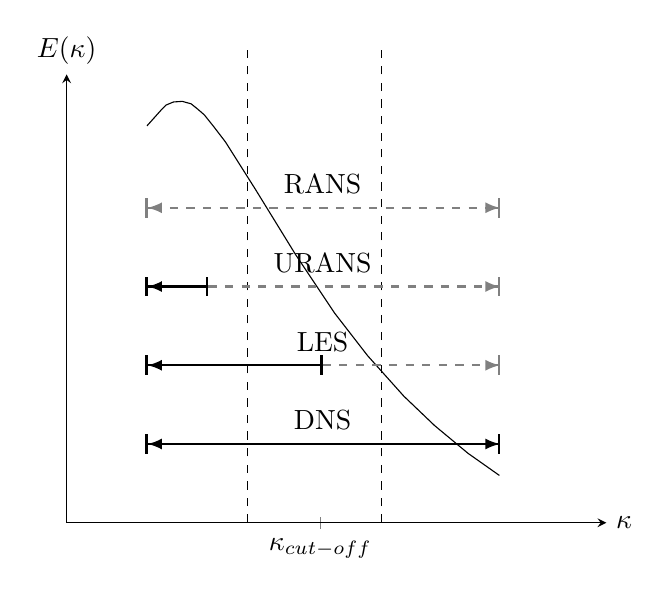
\begin{tikzpicture}
    \begin{axis}[
                %grid=both,
                ymin=0,
                ymax=1,
                xmax=1,
                xmin=0,
                xtick = 0.47,
                xticklabel=$\kappa _{\text{cut-off}}$,
                ytick = \empty,
                yticklabel=\empty,
                %minor tick num=1,
                axis lines = middle,
                xlabel=$\kappa$,
                ylabel=$E(\kappa)$,
                xlabel style={at=(current axis.right of origin), anchor=west},
                ylabel style={at=(current axis.above origin), anchor=south},
                %label style = {at={(ticklabel cs:1.1)}}
                ]
\end{axis}

\coordinate (B) at (6*0.17,                6*0.84);
\coordinate (F) at (6*0.200207468879668,   6*0.8737659643261302);
\coordinate (G) at (6*0.2105809128630705,  6*0.8841421027105674);
\coordinate (H) at (6*0.22614107883817425, 6*0.890615401196314);
\coordinate (I) at (6*0.24481327800829872, 6*0.8918898528857034);
\coordinate (J) at (6*0.2634854771784232,  6*0.8866707980815864);
\coordinate (K) at (6*0.2780082987551867,  6*0.8749636255860322);
\coordinate (L) at (6*0.2914937759336099,  6*0.8632578002909952);
\coordinate (M) at (6*0.3112033195020747,  6*0.8385568788058414);
\coordinate (N) at (6*0.3360995850622406,  6*0.8060570135258931);
\coordinate (P) at (6*0.39937759336099576, 6*0.7059748342943364);
\coordinate (Q) at (6*0.48340248962655596, 6*0.5695020746887967);
\coordinate (R) at (6*0.567427385892116,   6*0.4434189254728673);
\coordinate (S) at (6*0.6369294605809128,  6*0.3537182734278170);
\coordinate (T) at (6*0.7136929460580912,  6*0.2679042948752492);
\coordinate (U) at (6*0.7790456431535268,  6*0.2054817589049954);
\coordinate (V) at (6*0.8495850622406638,  6*0.1469485908282588);
\coordinate (W) at (6*0.9159751037344398,  6*0.1001091232419033);

%  \draw [gray!50]  (A) -- (B);
  \draw [] plot [smooth, tension=0.] coordinates {(B) (F) (G) (H) (I) (J) (K) (L) (M) (N) (P) (Q) (R) (S) (T) (U) (V) (W)};

  \draw [dashed] (2.3,0.) -- (2.3,6);
  \draw [dashed] (4.,0.) -- (4.,6);

  \draw [|latex-,thick] (1.,1.) -- (1.1,1);
  \draw [-|,thick] (5.4,1.) -- (5.5,1);
  \node at (3.25,1) [yshift=0.3cm] {DNS};
  \draw [-latex, thick] (1.,1.) -- (5.5,1);

  \draw [|latex-|,thick] (1.,2.) -- (3.25,2);
  \draw [-|,dashed, gray, thick] (5.4,2.) -- (5.5,2);
  \node at (3.25,2) [yshift=0.3cm] {LES};
  \draw [-latex,dashed, gray, thick] (3.25,2.) -- (5.5,2);

  \draw [|latex-|,thick] (1.,3.) -- (1.8,3);
  \draw [-|,dashed, gray, thick] (5.4,3.) -- (5.5,3);
  \node at (3.25,3) [yshift=0.3cm] {URANS};
  \draw [-latex,dashed, gray, thick] (1.8,3.) -- (5.5,3);

  \draw [|latex-,thick, gray, dashed] (1.,4.) -- (1.1,4);
  \draw [-|,dashed, gray, thick] (5.4,4.) -- (5.5,4);
  \node at (3.25,4) [yshift=0.3cm] {RANS};
  \draw [-latex,dashed, gray, thick] (1.1,4.) -- (5.5,4);

\end{tikzpicture}


   \caption{Energy spectrum showing the scales at which different computational models resolve (--) and model ({\color{gray}- -}) turbulence}
  \label{fig:modelling}
\end{figure}

%\begin{figure}[H]
%  \centering
%  \includegraphics[width=0.5\textwidth]{../Figures/Energy}
%  \caption{Modeling fraction of different turbulence models}\label{fig:modelling}
%\end{figure}




%
%   .--~*teu.
%  dF     988Nx
% d888b   `8888>
% ?8888>  98888F
%  "**"  x88888~
%       d8888*`
%     z8**"`   :
%   :?.....  ..F
%  <""888888888~
%  8:  "888888*
%  ""    "**"`
%
% http://patorjk.com/software/taag/#p=display&f=Fraktur  --  Text to ASCII graphics
%
%%%%%%%%%%%%%%%%%%%%%%%%%%%%%%%%%%%%
%%%%%%%%%%%%%%%%%%%%%%%%%%%%%%%%%%%%
\chapter{Methodology\label{ch:NM}}
Many of the simulations presented in this thesis were performed using G3D::Flow, a finite volume CFD solver for compressible flows that is developed and maintained in-house at the Division of Fluid Dynamics at Chalmers University of Technology. It is based on a family of codes developed by Eriksson\cite{g3dflow}, and uses the three-stage Runge-Kutta time marching method with a third-order accurate upwind-biased scheme for all convective terms and a second-order accurate compact centered scheme for all diffusive terms. For more details on the numerical scheme, see the work of Eriksson\cite{g3dflow} or Andersson et al.\cite{g3dflowNA}.

The governing equations are solved using G3D::Flow in conjunction with one of a range of different turbulence models depending on the level of detail needed from the simulation. In this project, the Spalart-Allmaras one equation turbulence model (SA) and the DDES model were implemented into the solver. The correctness of the implementation of the SA model in G3D::Flow is verified in Chapter \ref{ch:verification}, which compares the current solver to a well known and tested alternative. 
%
\section{Governing equations}
The CFD solver solves the governing equations for continuity, momentum, and energy presented in Eq. \ref{eq:NS}, which are commonly referred to as the Navier-Stokes equations. In compressible, unsteady and viscid form, they are:
\begin{equation} 
  \label{eq:NS}
  \begin{gathered}
    \frac{\partial {\rho}}{\partial t} + \frac{\partial \left({\rho} {u}_j \right)}{\partial x_j} = 0 \\
    \frac{\partial \left( {\rho} {u}_i \right)}{\partial t} + \frac{\partial\left({\rho} {u}_i {u}_j \right)}{\partial x_j} = -\frac{\partial p}{\partial x_i} + \frac{\partial {\sigma} _{ij}}{\partial x_j} \\
    \frac{\partial \left( {\rho} {e}_0\right)}{\partial t} + \frac{\partial \left({\rho} {e}_0 {u}_j\right)}{\partial x_j}= -\frac{\partial {p}{u}_j}{\partial x_j}+\frac{\partial}{\partial x_j}\left(C_p\frac{\mu}{Pr}\frac{\partial {T}}{\partial x_j}\right)+\frac{\partial}{\partial x_j}\left({u}_i\sigma_{ij}\right)
  \end{gathered}
\end{equation}
where ${\sigma} _{ij}$ is the viscous stress tensor
\begin{equation}
  {\sigma} _{ij} = \mu \left(2{S}_{ij}-\frac{2}{3}{S}_{mm}\delta _{ij}\right),
\end{equation}
${S}_{ij}$ is the strain rate tensor
\begin{equation}
  {S}_{ij}=\frac{1}{2}\left(\frac{\partial {u}_i}{\partial x_j}+\frac{\partial {u}_j}{\partial x_i}\right)
\end{equation}
and $Pr$ is the Prandtl number
\begin{equation}
  Pr = \frac{\mu C_p}{k}
\end{equation}
$C_p$ is the specific heat, $\mu$ the viscosity and k the thermal conductivity. The gas is assumed to be calorically perfect because all simulations reported in this thesis were performed under atmospheric conditions. This assumption implies that the gas obeys the ideal gas law and its internal energy and enthalpy are linear functions of the temperature
\begin{equation}
  \begin{aligned}
    e &= C_vT \\
    h &= C_pT \\
    C_v &= C_p-R
\end{aligned}
\end{equation}
To solve this set of equations, all scales down to the smallest Kolmogorov scales must be resolved (DNS). However, as discussed in the previous chapter, this would require the use of computationally unaffordable spatial and temporal resolutions. Limitations on available computational power thus mean that such approaches will not be practical for the foreseeable future. Consequently, modeling techniques are needed to close the set of equations. 

%The $\tau _{ij}$ is the turbulent stress term which models the momentum transport due to turbulence. It is this term that is solved dependent on which turbulence model is used, where resolving it results in high demands on the mesh- and time-scale of the simulation, hence DNS. This term is then modeled to some extent when using less computationally demanding turbulence models.\\
%\begin{equation}
%  \tau _{ij} = \mu _t 2{S}_{ij}
%\end{equation}

\section{URANS}
%Favre averaging
Time-averaging the governing equations has proven to be quite successful. For an arbitrary variable $\phi$ the averaging is expressed as
\begin{equation}
  \overline{\phi} = \lim\limits_{T \to \infty}\frac{1}{T}\int ^{T/2} _{T/2} \phi dt, \quad \phi = \overline{\phi}+\phi'
\end{equation}
where $\phi'$ denotes the fluctuating part of $\phi$. However, time-averaging the compressible form of the Navier-Stokes equations can produce quite cumbersome formulations. Therefore a density weighted averaging procedure (also known as Favre-averaging\cite{Favre1969}) can be used in conjunction with time-averaging. This has the advantage of reducing the number of terms in the averaged equations compared to the case for time-averaging alone. The Favre-averaging of a flow variable $\bar{\phi}$ is defined by the expression
\begin{equation}
  \hat{\phi} = \frac{\overline{\rho \phi}}{\bar{\rho}}
\end{equation}
with the instantaneous decomposition 
\begin{equation}
  \phi = \hat{\phi}+\phi'' = \frac{\overline{\rho \phi}}{\bar{\rho}}+\phi''
\end{equation}
where the $\phi''$ term represents the combination of the Reynolds decomposition fluctuating component $\phi'$ and the density fluctuations. The term $\bar{\phi}$ is the mean component of a specific variable. $\hat{\phi}$ and $\phi''$ can be thought of as low and high frequency components, respectively.
Applying both Favre-averaging and time-averaging to the governing equations yields the following expressions
\begin{equation} 
  \label{eq:NSFavre}
  \begin{gathered}
    \frac{\partial \overline{\rho}}{\partial t} + \frac{\partial \left(\overline{\rho} \hat{u}_j \right)}{\partial x_j} = 0 \\
    \frac{\partial \left( \overline{\rho} \hat{u}_i \right)}{\partial t} + \frac{\partial\left(\overline{\rho} \hat{u}_i \hat{u}_j \right)}{\partial x_j} = -\frac{\partial \overline{p}\delta _{ij}}{\partial x_i} + \frac{\partial \hat{\sigma} _{ij}}{\partial x_i}+\frac{\partial \tau _{ij}}{\partial x_j} \\
    \frac{\partial \left( \overline{\rho} \hat{e}_0\right)}{\partial t} + \frac{\partial \left(\overline{\rho} \hat{e}_0 \hat{u}_j\right)}{\partial x_j}= -\frac{\partial \overline{p}\hat{u}_j}{\partial x_j}+\frac{\partial}{\partial x_j}\left(C_p\frac{\mu}{Pr}\frac{\partial {T}}{\partial x_j}+q_j^t\right)+\frac{\partial}{\partial x_j}\left(\hat{u}_i\left(\overline{\sigma} _{ij} + \tau_{ij}\right)\right)\\
    -\frac{1}{2}\frac{\partial}{\partial x_j}\overline{\rho}\left(\widehat{u_iu_iu}_j-\widehat{u_iu}_i\hat{u}_j\right)
  \end{gathered}
\end{equation}
where $\hat{\sigma} _{ij}$ is the Favre-averaged viscous stress tensor
\begin{equation}
  \hat{\sigma} _{ij} = \mu \left(2\hat{S}_{ij}-\frac{2}{3}\hat{S}_{mm}\delta _{ij}\right),
\end{equation}
and $\hat{S}_{ij}$ is the Favre-averaged strain rate tensor
\begin{equation}
  \hat{S}_{ij}=\frac{1}{2}\left(\frac{\partial \hat{u}_i}{\partial x_j}+\frac{\partial \hat{u}_j}{\partial x_i}\right)
\end{equation}
It is immediately apparent that the Favre-averaged equations (Eqns. \ref{eq:NSFavre}) are very similar to the original Navier-Stokes equations (Eqns. \ref{eq:NS}). The triple velocity correlation term in the energy equation is neglected, leaving two additional terms - one for the turbulent stresses and one for the heat flux. The turbulent stress term, including the density, 
\begin{equation}
  \begin{aligned}
    \tau _{ij}  &= -\overline{\rho}\left(\widehat{u_iu}_j-\hat{u}_i\hat{u}_j\right)\\
                &= -\overline{\rho}\left(\underbrace{\left(\widehat{\hat{u}_i\hat{u}}_j-\hat{u}_i\hat{u}_j\right)}_I+\underbrace{\left(\widehat{u_i''\hat{u}}_j+\widehat{\hat{u}_iu''}_j\right)}_{II}+\underbrace{\widehat{u''_iu''}_j}_{III}\right)
  \end{aligned}
\end{equation}
consists of three different terms - the Leonard stresses term $I$, the cross stresses term $II$, and the Reynolds stresses term $III$. 

The turbulent heat flux is given by
\begin{equation}
  q_j^t = -C_p\overline{\rho}\left(\widehat{Tu}_j-\hat{T}\hat{u}_j\right) \label{eq:FavreEnd}
\end{equation}
This means that the closed set of equations formed by the Navier-Stokes equations is almost but not completely enclosed by the averaging technique, and the unknown turbulent stress terms must be modeled.

To evaluate the turbulent stress term and thereby close the set of equations, additional transport equations known as turbulence models are introduced. These equations solve for  one or more new variables. Many different models exist, but Spalart and Allmaras\cite{SA} derived a single equation turbulence model that assumes the turbulent stress is given by the expression
\begin{equation}
  \tau_{ij} = -2\nu_t{S}_{ij}
\end{equation}
where $\nu_t$ is the kinematic turbulent viscosity.

The SA model solves for a new turbulence variable, $\tilde{\nu}$. The conservative and compressible form of the model (without the $f_{t1}$ trip term) is as follows\cite{SA,SAmod}:
\begin{equation}
\begin{aligned}
  &\frac{\partial\bar{\rho}\tilde{\nu}}{\partial t}+\frac{\partial}{\partial x_j}\left(\bar{\rho}{u}_i{u}_j\right) = \tilde{S}\tilde{\nu}\left(1-f_{t2}\right)c_{b1}\bar{\rho}+\frac{1}{\sigma}\frac{\partial}{\partial x_j}\left(\bar{\rho} \left(\nu+\tilde{\nu}\right)\frac{\partial \tilde{\nu}}{\partial x_j}\right)\\
  &+\frac{c_{b2}}{\sigma}\bar{\rho}\left(\frac{\partial \tilde{\nu}}{\partial x_j}\right)^2-\bar{\rho}\left(c_{w1}f_w-\frac{c_{b1}}{\kappa ^2}f_{t2}\right)\left(\frac{\tilde{\nu}}{d}\right)^2+\frac{1}{\sigma}\left(\nu+\tilde{\nu}\right)\frac{\partial \bar{\rho}}{\partial x_j}\frac{\partial \tilde{\nu}}{\partial x_j}\label{eq:SA}
\end{aligned}
\end{equation}
where  
\begin{equation}
  \begin{gathered}
    \nu_t = \tilde{\nu}f_{v1}, \qquad f_{v1}=\frac{\chi^3}{\chi^3+c_{v1}^3},\qquad \chi = \frac{\tilde{\nu}}{\nu}\\
  \tilde{S} = S + \frac{\tilde{\nu}}{\kappa ^2 d ^2}f_{v2}, \qquad f_{v2}=1-\frac{\chi}{1+\chi f_{v1}}\\
  f_w=g\left(\frac{1+c_{w3}^6}{g^6+c_{w3}^6}\right)^{1/6},\quad g=r+c_{w2}\left(r^6-r\right), \quad r=\frac{\tilde{\nu}}{\tilde{S}\kappa^2d^2}\\
    f_{t2} = c_{t3}exp\left(-c_{t4}\chi^2\right)\label{eq:SAf}
  \end{gathered}
  \end{equation}
and the corresponding constants are
\begin{equation}
  \begin{aligned}
    &c_{b1}=0.1355, &\sigma=2/3,\qquad  &c_{b2}=0.622,\qquad &\kappa=0.41, \\
    &c_{w2}=0.3,    &c_{w3}=2,  \qquad  &c_{v1}=7.1,  \qquad  &c_{t3}=1.2, \\
    &c_{t3}=0.5,  &  &c_{w1}=c_{b1}/\kappa^2+\left(1+c_{b2}\right)/\sigma.
  \end{aligned}
\end{equation}
In the SA model, the turbulence stress term $\tau _{ij}$ (referred to as the Reynolds stress term in RANS models) accounts for the effects of the entire energy spectrum over all length scales in the average flow field. This means that all turbulence is modeled. 

\section{LES}
The LES equations are written in the same way as the governing equations of URANS except that instead of applying a time-averaging technique, spatial filtering is used. This means that for a filtered arbitrary variable $\phi$,
\begin{equation}
  \overline{\phi}(x,t) = \frac{1}{\Delta x}\int ^{x+0.5\Delta x} _{x-0.5\Delta x} \phi(\xi,t) d\xi, \quad \phi = \overline{\phi}+\phi'
\end{equation}
Therefore, Eqns \ref{eq:NSFavre}-\ref{eq:FavreEnd} can be regarded as the Favre-averaged LES governing equations, with the modification that $\left(\bar{\bullet}\right)$ represents spatial filtering instead of time-averaging. Furthermore, because finite volume discretization is used in LES, the local control volume based on the computational grid represents the spatial filtering (i.e. an implicit filter is used). This means that the difference between RANS and LES is the extent to which the Reynolds stresses are modeled (which is much greater for RANS). Additionally, LES models describe turbulent stresses in a different way to RANS: the stresses that are not resolved are modeled using SGS models, the simplest of which is the zero-equation Smagorinsky model\cite{Smagorinsky}:
\begin{equation}
  \begin{aligned}  \tau_{ij} - \frac{1}{3}\delta_{ij}\tau_{kk} &= -\nu_{sgs}\left(\frac{\partial \overline{u}_i}{\partial x_j}+\frac{\partial \overline{u}_j}{\partial x_i}\right) = -2\nu_{sgs}\overline{S}_{ij}\\
  \nu_{sgs} &=\left(C_S\Delta \right)^2\sqrt{2\overline{S}_{ij}\overline{S}_{ij}} \equiv \left(C_S\Delta \right)\left|\overline{S}\right|
  \end{aligned}
\end{equation}
Additionally, the filter-width is defined as the local grid size:
\begin{equation}
  \Delta = \left(\Delta V_{IJK}\right)^{1/3}
\end{equation}
As described in Chapter \ref{ch:Intro} the SGS are defined by the cut-off wavelength; length-scales below the cut-off are modeled, while those above it are resolved. Consequently, the use of finer meshes reduces the proportion of the energy spectrum that is modeled, which can make common mesh-dependency studies difficult. LES simulations are also quite computationally demanding because the larger scales become quite small in the vicinity of walls, necessitating the use of a fine mesh and a small timestep.

\section{DDES}
The preceding sections describe the URANS and LES formulations. A new class of hybrid turbulence modeling techniques known as hybrid LES/RANS methods has recently been introduced with the aim of combining the best aspects of the URANS and LES approaches. The hybrid models simulate certain regions (typically, attached or mildly separated boundary layers) using the URANS formulation of the governing equations, while the free-stream region and well-separated areas are solved using LES. The transition between URANS and LES can be predefined (using so-called zonal methods) and calculated as a part of the model. This means that the boundary layer, for which URANS models have proven quite reliable, can use a relatively coarse mesh, substantially reducing computational costs because fewer cells and a larger time-step can be used. Using the LES in the free-stream means that transient flow features of the main flow are captured much better than they would be by the URANS model, which uses a lower degree of modeling.

The hybrid LES/RANS model DDES is based on the original Detached Eddy Simulation (DES) model\cite{DES97}. It uses the SA one-equation turbulence model in URANS mode and as a SGS model for the LES region. To implement the SA model as a SGS model, the destruction term of an SA-model length scale was modified to account for the change from RANS to LES. To achieve this, the wall distance for the SA model was replaced with a different length scale, as shown in Eq. \ref{eq:DDES}. In other words, the wall distance, $d$, in Eqns. \ref{eq:SA} and \ref{eq:SAf} is replaced by $\tilde{d}$ in Eq. \ref{eq:DDES}. DDES is an improvement over the original DES model because the switching between LES and RANS is governed by both the cell size and the flow itself. This has great benefits because the original DES model had a high risk of premature switching from RANS to LES for grids with a stream-wise grid spacing similar in size to the boundary layer thickness. Such premature switching causes grid-induced separation\cite{DDES}, which has particularly severe effects in simulations of flows with strong gradients in the stream-wise direction: if the stream-wise grid size is similar in size to the boundary layer thickness, the original DES model extends the LES region into the boundary layer, where the grid is not fine enough to resolve the turbulent stresses. This problem was addressed in the DDES model by adding a shielding function that prevents the application of the LES formulation to the boundary layer. The shielding function,
\begin{equation}
  f_d = 1-\tanh\left[(8r_d)^3\right].
  \label{eq:fd}
\end{equation}
is designed to be 0 in the boundary layer but 1 outside it. The function $r_d$ is similar to the $r$ function in the SA model\cite{SA}
\begin{equation}
  r_d = \frac{\nu+\nu_t}{\sqrt{U_{i,j}U_{i,j}}\kappa^2 d^2}
  \label{eq:rd}
\end{equation}
The length scale introduced in the original DES model was based only on the wall distance and the grid spacing $\Delta$:
\begin{equation}
  \tilde{d}=min(d,C_{DES}\Delta)
  \label{eq:DES97}
\end{equation}
However, as noted above, this can cause grid-induced separation. To eliminate this problem, the DDES model uses a modified length scale incorporating a boundary layer shielding function, $f_d$: 
\begin{equation}
  \tilde{d} = d-f_dmax(0,d-C_{DES}\Delta).
  \label{eq:DDES}
\end{equation}
When $f_d=0$, the model behaves like a RANS model, but when $f_d=1$, it behaves like the original DES model shown in Eq.~(\ref{eq:DES97}). Outside the boundary layer, the DES model should be in LES mode. Shur et al.\cite{DES99} compared the output of the original DES model using the SA model to describe SGS behavior to experimental results and the output of the DES model used in conjunction with the Smagorinsky SGS model. Good achievement with experimental results was achieved when simulating isotropic turbulence using a filtering factor value of $C_{DES}=0.65$.

The coefficients of the $f_d$ function were calibrated using a flat-plate boundary layer, but recent studies have shown that some modifications may be necessary for it to perform well for specific problems. For example, Ashton\cite{Ashton2016} encountered problems with the shielding function during studies on a three-element airfoil. It was concluded that these problems were due to excessively fine stream-wise and span-wise grid sizes, even though the DDES model was used. The fine mesh created strong pressure gradients over curved surfaces and caused the shielding function to break down, allowing the LES model to be applied inside the boundary layer. Probst et al.\cite{Probst2010} encountered a similar problem in studies on a simple airfoil. In their opinion, a coarser mesh was not a viable option because a high resolution in the stream-wise direction was required to capture the adverse pressure gradient over the wing. Instead, they suggested a slight modification to the $f_d$ function whereby the value of the coefficient in front of $r_d$ was increased from 8 to 16, as shown in Eq. \ref{eq:fdmod}. 
\begin{equation}
  f_d = 1-\tanh\left[(16r_d)^3\right].
  \label{eq:fdmod}
\end{equation}
This shows that despite the implementation of modifications to allow the DDES model to cope with ambiguous grids, the solutions remain sensitive to stream-wise grid spacing. The shielding function of  the DDES model was designed to shield the boundary layer independently of the mesh. To find optimal settings for simulations of PSW modules, both versions of the $f_d$ function were tested and evaluated for a single PSW module, indicating that the modified function performs better in this case [Paper \ref{pap:SciTech18}]. However, further studies are needed to confirm this conclusion.

It has also been shown that when using the SA model as a base model for DDES, $f_{t2}$ should not be included in the equations because it increases the likelihood that the boundary layer will remain laminar over the geometry on finer grids\cite{Vatsa2017}.

Figure \ref{fig:FPDDES} shows how the DDES approach results in the application of different modeling techniques in different regions when simulating a flow over an inclined flat plate. In the figure, the free-stream and the separated region on the suction side are solved using LES while the attached boundary layer on the pressure side is solved using RANS.
\begin{figure}[H]
  \centering
%\documentclass[12pt,english]{article}
%\usepackage{fullpage}
%\usepackage[T1]{fontenc} 
%\usepackage{helvet}
%\renewcommand{\familydefault}{\sfdefault}
%\usepackage{babel}
%\usepackage{amsmath}
%\numberwithick{equation}{section}
%\usepackage{hyperref}
%\usepackage{tikz,pgfplots}
%\usepackage{boldline} %To get thicker lines in tables
%\usepackage{float}    %For float on figures for exampel
%\usepackage{graphicx} %Figures
%
%\usepackage{sectsty}
%\allsectionsfont{\centering}
%
%\renewcommand{\thesubsection}{\Roman{subsection}} 
%\renewcommand{\thesubsubsection}{\Alph{subsubsection}} 
%
%\newcommand{\ignore}[1]{}
%\def\circledarrow#1#2#3{ % #1 Style, #2 Center, #3 Radius
%  \draw[#1,->] (#2) +(80:#3) arc(80:-260:#3);
%}
%
%\begin{document}
%
%\begin{figure}[H]
%  \centering
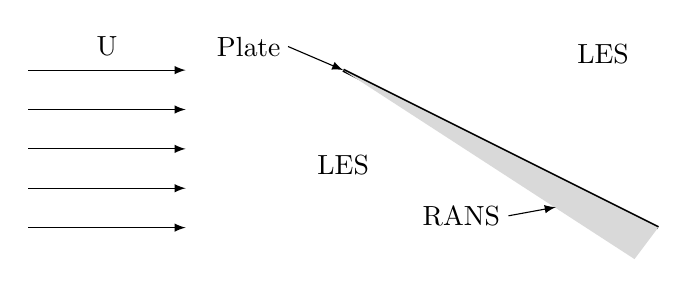
\begin{tikzpicture}
  \coordinate (A) at (0,0);
  \coordinate (B) at (2,0);
  \coordinate (C) at (0,0.5);
  \coordinate (D) at (2,0.5);
  \coordinate (E) at (0,1);
  \coordinate (F) at (2,1);
  \coordinate (G) at (0,1.5);
  \coordinate (H) at (2,1.5);
  \coordinate (I) at (0,2);
  \coordinate (J) at (2,2);
  %Arrows
  \draw[-latex] (A)--(B);
  \draw[-latex] (C)--(D);
  \draw[-latex] (E)--(F);
  \draw[-latex] (G)--(H);
  \draw[-latex] (I)--(J);
  %Plates
  \coordinate (AA) at (4,2);
  \coordinate (BB) at (8,0);
  \coordinate (CC) at (7.7,-0.4);
  \draw[very thick] (AA)--(BB);
  \fill[gray!30] (AA) -- (BB) -- (CC) -- cycle;
  %circles - First
  \circledarrow{thick, gray}{4.3,2}{0.1cm};
  \circledarrow{thick, gray}{4.65,1.95}{0.1cm};
  \circledarrow{thick, gray}{4.95,1.7}{0.1cm};
  \circledarrow{thick, gray}{5.4,1.5}{0.1cm};
  \circledarrow{thick, gray}{5.9,1.3}{0.1cm};
  \circledarrow{thick, gray}{6.3,1.1}{0.1cm};
  \circledarrow{thick, gray}{6.7,0.95}{0.1cm};
  \circledarrow{thick, gray}{7.1,0.7}{0.1cm};
  \circledarrow{thick, gray}{7.5,0.5}{0.1cm};
  \circledarrow{thick, gray}{8.0,0.3}{0.1cm};
  %Circles - second
  \circledarrow{thick, gray}{5.2,1.85}{0.15cm};
  \circledarrow{thick, gray}{5.7,1.7}{0.15cm};
  \circledarrow{thick, gray}{6.2,1.5}{0.15cm};
  \circledarrow{thick, gray}{6.6,1.3}{0.15cm};
  \circledarrow{thick, gray}{6.9,1.8}{0.15cm};
  \circledarrow{thick, gray}{7.2,1.0}{0.15cm};
  \circledarrow{thick, gray}{7.8,0.8}{0.15cm};
  \circledarrow{thick, gray}{8.2,0.95}{0.15cm};
  %Circle - third
  \circledarrow{thick, gray}{6.4,1.9}{0.2cm};
  \circledarrow{thick, gray}{7.0,1.45}{0.2cm};
  \circledarrow{thick, gray}{7.5,1.6}{0.2cm};
  \circledarrow{thick, gray}{7.8,1.2}{0.2cm};
  \circledarrow{thick, gray}{8.3,1.5}{0.2cm};
  
  \node at (1,2.3) {U};
  \node at (4,0.8)  {LES};
  \node at (7.3,2.2)  {LES};
  \node at (5.5,0.15) {RANS};
  \node at (2.8,2.3)  {Plate};

  \draw [-latex] (3.3,2.3)--(4.0,2.0);
  \draw [-latex] (6.1,0.15)--(6.7,0.26);
  %\draw[step=0.1cm,gray,very thick] (4,0) grid (9,2);

\end{tikzpicture}
%  \caption{???}
%  \label{fig:zones}
%\end{figure}
%\end{document}

  \caption{An inclined flat plate simulated with DDES}\label{fig:FPDDES}
\end{figure}


%   .x~~"*Weu.
%  d8Nu.  9888c
%  88888  98888
%  "***"  9888%
%       ..@8*"
%    ````"8Weu
%   ..    ?8888L
% :@88N   '8888N
% *8888~  '8888F
% '*8"`   9888%
%   `~===*%"`
%
%%%%%%%%%%%%%%%%%%%%%%%%%%%%%%%
%%%%%%%%%%%%%%%%%%%%%%%%%%%%%%%
\chapter{Unpublished results\label{ch:sim}}%Computaional model of the experimental rig\label{ch:sim}}
Performing simulations on a computational model representing the experimental ICD test rig requires a high quality grid and predefined boundary conditions. The sections below introduce the computational domain of the simulations presented in this thesis and the setup of those simulations.
%
\section{Computational domain}
Figure \ref{fig:rig} shows the computational domain of the simulations. It is a 3D-extension of the setup presented in Figure \ref{fig:schema}, with the casing walls and bleed pipe removed for the sake of visibility. As discussed in Chapter \ref{ch:Intro}, the domain is divided into four main modules: the PSW, bleed pipe, OGV, and ICD.
\begin{figure}[H]
  \centering
  \begin{tikzpicture}
    \node[anchor=south west,inner sep=0] at (0,0) {\includegraphics[width=9.05cm]{Figures/RigBladesAndSurfaces.pdf}};
  \node at (3.3,5.4) {\bf{FT}};
  \draw[-latex] (3.0,5.4)--(2.65,5.0);
  \node at (4.05,5) {\bf{P$_\text{OGV}$}};
  \draw[-latex] (3.5,5)--(3.1,4.65);
  \node at (5.6,3.9) {\bf{P$_\text{DUCT}$}};
  \draw[-latex] (4.9,3.9)--(4.36,3.36);
  \node at (6.8,3.) {\bf{NRT}};
  \draw[-latex] (6.8,2.8)--(6.57,2.2);
  \node at (7.8,2.4) {\bf{FRT}};
  \draw[-latex] (7.8,2.2)--(7.54,1.8);
  \node at (3.6,1.1) {\bf{Strut}};
  \draw[-latex] (3.7,1.2)--(4,1.6);
    \node at (1.9,1.2) {\bf{OGV}};
  \draw[-latex] (1.9,1.4)--(2.2,1.8);
  \node at (0.3,3.8) {\bf{PSW}};
  \draw[-latex] (0.5,4.0)--(0.9,4.4);
    %\draw[help lines,step=.2] (0,0) grid (8.5,6);
\end{tikzpicture}
  \caption{3D representation of the computational domain}\label{fig:rig}
\end{figure}

To account for all the interactions between different modules and blades, all domains must have an equal pitch. The ICD module is the widest of the modules, and covers a 40$^{\circ}$ tangential sector, so all the other modules must be implemented with the same sector width. Consequently, 5 PSWs, 9 OGVs and 1 strut were included in the CFD analysis. Figures \ref{fig:meshPSW}-\ref{fig:meshDuct} show the meshes for the leading and trailing edges of the PSWs, OGVs, and strut. They are all multi-block structured meshes with an O-grid around the blades to establish a well-resolved boundary layer.

\begin{figure}[h!]
  \centering
  \begin{minipage}{0.49\columnwidth}
  \includegraphics[width=6cm]{Figures/Leadingedge.pdf}
  \end{minipage}
  \begin{minipage}{0.49\columnwidth}
  \includegraphics[width=6cm]{Figures/Trailingedge.pdf}
  \end{minipage}
  \caption{Leading and trailing edge meshes for the PSWs.} \label{fig:meshPSW}
\end{figure}
\begin{figure}[h!]
  \begin{minipage}{0.49\columnwidth}
  \includegraphics[width=6cm]{Figures/Leadingedge.pdf}
  \end{minipage}
  \begin{minipage}{0.49\columnwidth}
  \includegraphics[width=6cm]{Figures/Trailingedge.pdf}
  \end{minipage}
  \caption{Leading and trailing edge meshes for the OGVs.} \label{fig:meshOGV}
\end{figure}
\begin{figure}[h!]
  \begin{minipage}{0.49\columnwidth}
  \includegraphics[width=6cm]{Figures/DuctLeadingedge.pdf}
  \end{minipage}
  \begin{minipage}{0.49\columnwidth}
  \includegraphics[width=6cm]{Figures/DuctTrailingedge.pdf}
  \end{minipage}  
  \caption{Leading and trailing edge meshes for the strut.} \label{fig:meshDuct}
\end{figure}
%
The bleed pipe is axisymmetric and is therefore relatively simple to mesh. The 2D mesh, shown in Figure \ref{fig:bleed}, is rotated around the common ICD axis to obtain the 3D mesh. During this procedure, the bleed module is adjusted to match the tangential sectors of the surrounding modules. The bleed pipe module is connected to the PSWs on the upstream side and the OGVs on the downstream side. The bleed pipe outlet is located on the upper surface of the module. The mesh was generated using an in-house meshing tool called G3dmesh. Because the SA turbulence model was used and the risk of separation was expected to be high, the boundary layer was resolved with $y^+\approx1-3$.

\begin{figure}[H]
  \centering
    \begin{tikzpicture}
      \node[anchor=south west,inner sep=0] at (0,0) {    \includegraphics[width=9.05cm, height=6cm]{Figures/BleedGrid2D.pdf}};
      \node at (7.2,6.15) {\bf{Bleed pipe outlet}};
      \node at (0.1,1.8) {\bf{PSW}};
      \node at (5.8,1.8) {\bf{OGV}};
    %\draw[help lines,step=.2] (0,0) grid (9,6);
    \end{tikzpicture}
\caption{2D representation of the bleed pipe mesh.}\label{fig:bleed}
\end{figure}


\section{Computational setup}
A General Grid Interface (GGI) was used to calculate the fluxes between the different modules, i.e. the PSWs, bleed pipe, OGVs, and duct. This was done to ensure that all wakes and transient phenomena were transported from upstream modules to downstream ones. The applied boundary conditions were obtained from earlier 1D calculations. At the inlet boundary, the total temperature and pressure are specified together with the direction of the velocity. The bleed pipe outlet was specified to have a constant static pressure, whereas the duct's outlet was specified in terms of the mass flow. Predefining the massflow at the outlet forces the solution towards the correct throughflow. The total temperature and the free stream SA viscosity for the inlet boundary were identical for all bleed fractions; the temperature was set to a normal atmospheric temperature, and $\tilde{\nu}_{in}$ was set to $5\nu$. The latter value corresponds to a relatively low turbulence intensity. However, because the main purpose of the simulations was to analyze the duct’s performance, it was assumed that the PSW would be sufficient to generate a highly turbulent flow, and that the inlet boundary would therefore have little effect on the results obtained. The pressure and massflow data used in the simulations cannot be presented for reasons of confidentiality.
%%%%%%%
%%%
%%% Editor's note:
%%% We would be specify precisely what is meant by a 'normal atmospheric temperature', for example by changing the phrase to 'a normal atmospheric temperature of XXX K'.
%%%
%%%%%%%%

Both solvers were used to simulate two different operating conditions. The first operating condition was a low bleed fraction scenario in which $10\%$ of the inlet massflow was extracted through the bleed pipe. The second was a high bleed fraction scenario in which $40\%$ of the inlet massflow was extracted. The two cases have the same inlet boundary condition but different bleed outlet pressures and mass flows through the duct. 

%\begin{table}[H]
%  \caption{Boundary conditions} \label{tab:bc}
%  \centering
%\begin{tabular}{|c|c|c|c|c|c|}
%  \hline
%  \multicolumn{2}{|c|}{$\dot{m}_{bleed}=0.1$} & \multicolumn{2}{|c|}{$\dot{m}_{bleed}=0.4$} & \multicolumn{2}{|c|}{$\dot{m}_{bleed}=0.5$}\\
%  \hlineB{2}
%  $p_{in}$    & ?????   & $p_{in}$    & ????? & $p_{in}$    & ?????\\
%  \hline                                                           
%  $p_{t,in}$  & ?????   & $p_{t,in}$  & ????? & $p_{t,in}$  & ?????\\
%  \hline                                                           
%  $p_{out}$   & ?????   & $p_{out}$   & ????? & $p_{out}$   & ?????\\
%  \hline
%  $u_{in}$    & ?????   & $u_{in}$    & ????? & $u_{in}$    & ????? \\
%  \hline
%%  $T_{t,in}$          & 280     &               &      \\
%%  \hline
%%  $\tilde{\nu}_{in}$  & 5$\nu$  &               &      \\
%%  \hline
%\end{tabular}
%\end{table}

\section{Computational comparison}
This section compares results obtained in simulations of the complete experimental test rig using the in-house G3D::Flow solver to the results of equivalent simulations performed using the commercial solver CFX. These comparisons, together with those presented in Paper \ref{pap:ASME18}, provide valuable insights into the in-house solver's performance and increase confidence in its output.

The outputs of the two solvers are visualized in the form of radial profiles of the Mach number, total pressure, and pressure at the front traverse (FT), near rear traverse (NRT), and far rear traverse (FRT) surfaces, and the wall pressure at the intersection between the P$_\text{DUCT}$ and the hub and casing. The locations of these surfaces and the intersection are displayed in Figure \ref{fig:rig}. The radial profiles for the Mach number, total pressure, and pressure were normalized against the corresponding maxima; the Mach number and total pressure were massflow averaged, but the pressure was area averaged. 

Figure \ref{fig:FT10} shows the radial profiles for the static and total pressures and the Mach number obtained with the in-house and commercial solvers for the $10\%$ bleed case at the FT surface. The two solvers agree very well: the two pressure profiles are almost identical, while the Mach number profiles and the total pressure profiles differ only with respect to some insignificant variation near the hub.
\begin{figure}[h!]
  \centering
  \begin{minipage}{0.48\columnwidth}
  \includegraphics[width=1.\textwidth]{Figures/MaMave_FT.png}
%    \caption*{Mach number.}
  \end{minipage}
  \begin{minipage}{0.48\columnwidth}
  \includegraphics[width=1.\textwidth]{Figures/PAave_FT.png}
%    \caption*{Static pressure.}
  \end{minipage}
  \begin{minipage}{0.48\columnwidth}
  \includegraphics[width=1.\textwidth]{Figures/P0Mave_FT.png}
%    \caption*{Total pressure.}
  \end{minipage}
  \caption{Radial profiles obtained with the CFX and G3D::Flow solvers for the Mach number (left), pressure, (right), and total pressure (bottom)  at the FT surface in the $10\%$ bleed fraction case.} \label{fig:FT10}
\end{figure}

The agreement between the two solvers became worse upon moving downstream through the S-shaped duct to the NRT surface, as shown in Figure \ref{fig:NRT10}. Although both solvers predicted the same major trends in the studied variables, there were noticeable differences in their predictions of the Mach number and total pressure for the region in the upper half of the duct. This could be due to differences in the predicted effects of the OGV wakes. Both solvers produced quite similar pressure profiles.

\begin{figure}[h!]
  \centering
  \begin{minipage}{0.48\columnwidth}
  \includegraphics[width=1.\textwidth]{Figures/MaMave_NRT.png}
%    \caption*{Mach number.}
  \end{minipage}
  \begin{minipage}{0.48\columnwidth}
  \includegraphics[width=1.\textwidth]{Figures/PAave_NRT.png}
%    \caption*{Static pressure.}
  \end{minipage}
  \begin{minipage}{0.48\columnwidth}
  \includegraphics[width=1.\textwidth]{Figures/P0Mave_NRT.png}
%    \caption*{Total pressure.}
  \end{minipage}
  \caption{Radial profiles obtained with the CFX and G3D::Flow solvers for the Mach number (left), pressure (right), and total pressure (bottom) at the NRT surface in the $10\%$ bleed fraction case.} \label{fig:NRT10}
\end{figure}
Figure \ref{fig:FRT10} shows the corresponding radial profiles for the FRT surface in the 10\% bleed fraction case. As was seen for the NRT surface, the Mach number and total pressure profiles obtained with the two solvers differ in the upper half of the duct. Once again, this can be attributed to differences in the predicted effects of the OGV wakes. The pressure profiles for the two solvers are similar, although they differ more markedly than at the other two surfaces in the $10\%$ bleed case.

Overall, the two solvers compare well for the $10\%$ bleed fraction case, albeit with some discrepancies in the predicted Mach number and total pressure profiles at the NRT and FRT surfaces in the upper half of the duct. This behavior might be explained by differences in the prediction of the OGV wakes; the duct's S-shaped curvature means that downstream of the strut, OGV wake effects are strongest in the upper half of the duct, affecting both local velocities and losses.

\begin{figure}[h!]
  \centering
  \begin{minipage}{0.48\columnwidth}
  \includegraphics[width=1.\textwidth]{Figures/MaMave_FRT.png}
%    \caption*{Mach number.}
  \end{minipage}
  \begin{minipage}{0.48\columnwidth}
  \includegraphics[width=1.\textwidth]{Figures/PAave_FRT.png}
%    \caption*{Static pressure.}
  \end{minipage}
  \begin{minipage}{0.48\columnwidth}
  \includegraphics[width=1.\textwidth]{Figures/P0Mave_FRT.png}
%    \caption*{Total pressure.}
  \end{minipage}
  \caption{Radial profiles obtained with the CFX and G3D::Flow solvers for the Mach number (left), pressure (right), and total pressure (bottom) at the FRT surface in the $10\%$ bleed fraction case.} \label{fig:FRT10}
\end{figure}

Figures \ref{fig:FT40}-\ref{fig:FRT40} show the corresponding radial profiles obtained with the commercial (CFX) and in-house (G3D::Flow) solvers for the $40\%$ bleed fraction case. For both solvers, the profiles obtained for the FT surface (see Figure \ref{fig:FT40}) under these conditions closely resemble those generated for the 10\% bleed fraction case. This was expected because differences in the bleed fraction should primarily affect the flow field downstream of the bleed pipe. As in the 10\% bleed fraction case, there were only minor and non-significant differences between the two solvers in terms of the Mach number, pressure, and total pressure profiles for the FT surface. However, there were significant differences between the profiles for all three variables generated by the two solvers at the other two surfaces in the 40\% bleed fraction case. Additionally, the higher level of bleed introduced some instability that made it difficult to obtain fully converged solutions. The general shapes of the profiles predicted by the two solvers are fairly similar; the most pronounced differences are observed for the Mach number and total pressure profiles at the FRT casing.
%
\begin{figure}[h!]
  \centering
  \begin{minipage}{0.48\columnwidth}
  \includegraphics[width=1.\textwidth]{Figures/MaMave_FT.png}
%    \caption*{Mach number.}
  \end{minipage}
  \begin{minipage}{0.48\columnwidth}
  \includegraphics[width=1.\textwidth]{Figures/PAave_FT.png}
%    \caption*{Static pressure.}
  \end{minipage}
  \begin{minipage}{0.48\columnwidth}
  \includegraphics[width=1.\textwidth]{Figures/P0Mave_FT.png}
%    \caption*{Total pressure.}
  \end{minipage}
  \caption{Radial profiles obtained with the CFX and G3D::Flow solvers for the Mach number (left), pressure (right), and total pressure (bottom) at the FT surface in the $40\%$ bleed fraction case.} \label{fig:FT40}
\end{figure}

\begin{figure}[h!]
  \centering
  \begin{minipage}{0.48\columnwidth}
  \includegraphics[width=1.\textwidth]{Figures/MaMave_NRT.png}
%    \caption*{Mach number.}
  \end{minipage}
  \begin{minipage}{0.48\columnwidth}
  \includegraphics[width=1.\textwidth]{Figures/PAave_NRT.png}
%    \caption*{Static pressure.}
  \end{minipage}
  \begin{minipage}{0.48\columnwidth}
  \includegraphics[width=1.\textwidth]{Figures/P0Mave_NRT.png}
%    \caption*{Total pressure.}
  \end{minipage}
  \caption{Radial profiles obtained with the CFX and G3D::Flow solvers for the Mach number (left), pressure (right), and total pressure (bottom) at the NRT surface in the $40\%$ bleed fraction case.} \label{fig:NRT40}
\end{figure}

\begin{figure}[h!]
  \centering
  \begin{minipage}{0.48\columnwidth}
  \includegraphics[width=1.\textwidth]{Figures/MaMave_FRT.png}
%    \caption*{Mach number.}
  \end{minipage}
  \begin{minipage}{0.48\columnwidth}
  \includegraphics[width=1.\textwidth]{Figures/PAave_FRT.png}
%    \caption*{Static pressure.}
  \end{minipage}
  \begin{minipage}{0.48\columnwidth}
  \includegraphics[width=1.\textwidth]{Figures/P0Mave_FRT.png}
%    \caption*{Total pressure.}
  \end{minipage}
  \caption{Radial profiles obtained with the CFX and G3D::Flow solvers for the Mach number (left), pressure (right), and total pressure (bottom) at the FRT surface in the $40\%$ bleed fraction case.} \label{fig:FRT40}
\end{figure}
Figure \ref{fig:duct10} shows the two solvers' predictions of the normalized static pressure at the intersection between the P$_\text{DUCT}$ and the endwalls in the $10\%$ bleed case. The plotted pressures are normalized against the total pressure at the inlet, and the pressure is shown as a function of the location along the x-axis, normalized against the distance from the leading edge of the duct to the duct's outlet. The vertical dashed lines indicate the x-locations of the strut's leading and trailing edges. The two solvers' pressure predictions agree well at the hub, with only minor deviations in the minimum value. However, closer to the casing, the results obtained using G3D::Flow fluctuate more strongly than those obtained with CFX. %This might be caused by the fact that the CFX solver is designed to kill all minor fluctuations in the flow. 

Data on the wall pressure in the S-shaped duct are not presented for the $40\%$ bleed case because strong pressure fluctuations at the walls made it impossible to meaningfully compare the two solvers. The reason for this is discussed in Paper \ref{pap:ASME18}; it is related to the shortness of the bleed pipe, which gave rise to pressure fluctuations that affected the flow.
\begin{figure}[h!]
  \centering
  \includegraphics[width=.8\textwidth]{Figures/CFXG3dDuct10.png}
    \caption{Normalized pressure at the ICD.} \label{fig:duct10}
\end{figure}

% 88        88
% 88        88
% 88        88
% 88        88
% 88        88
% 888888888888
%           88 
%           88 
%           88 
%           88
%           88  
%           
%%%%%%%%%%%%%%%%%%%%%%%%%%%%%%%
%%%%%%%%%%%%%%%%%%%%%%%%%%%%%%%
\chapter{SA turbulence model verification\label{ch:verification}}
To verify that the SA turbulence model was implemented correctly, a zero gradient boundary layer build up over a flat plate was simulated. Because the SA model is a low Reynolds number model a $y^+ \approx 1$ was targeted and steps were taken to ensure there were at least 10 cells inside the boundary layer so that the boundary layer would be well-resolved. These objectives were achieved for most of the tested grids, but the $y^+$ value for the grid with the lowest cell count was slightly above the target.\\
A grid dependency study was performed and the results obtained with the CF3D solver were compared to data obtained from the NASA Turbulence Model Resources\cite{NASA}. The drag coefficient $C_D$ was used in the grid dependency analyses:
\begin{equation}
C_D=\frac{2F_D}{\rho_{ref}U^2_{ref}A}
\label{eq:CD}
\end{equation}
Here, $F_D$ is the drag force, $\rho_{ref}$ is a reference density, $U_{ref}$ is a reference velocity, and $A$ is the surface in contact with the fluid.\\
The skin friction coefficient, $C_f$, was also used in the grid dependency study to compare the two solvers. The skin friction coefficient is defined as
\begin{equation}
  C_f = \frac{2\tau _w}{\rho_{ref}U^2_{ref}}
  \label{eq:CF}
\end{equation}
where $\tau _w$ is the wall shear stress
\begin{equation*}
  \tau_w = \mu \left( \frac{\partial u}{\partial y}\right)_{y=0}
\end{equation*}
$\mu$ is the dynamic viscosity, u is the flow parallel to the wall and y is the distance to the wall.

\section{Flat plate simulation}
The computational domain for the 2D flat plate boundary layer build up simulations is depicted in Figure \ref{fig:FP}. The geometry of the system and its various boundaries are also shown. The symmetry boundary located between $x = -0.4$ and $x = 0$ is there to ensure that the inlet boundary will not be affected by the viscous wall.
\begin{figure}[H]
  \centering
\begin{tikzpicture}
\begin{axis}[
  axis x line=bottom,
  axis y line=left,
%  scale only axis,
  xtick={-0.4,-0.2,...,2.1},
  ytick={-0.1,0,0.2,...,1.,1.1},
  xlabel={$\bf{x}$},
  ylabel={$\bf{y}$},
  xlabel style={below right},
  ylabel style={above left,rotate= -90},
  x=5cm,
  xmin=-0.4,
  xmax=2.1,
  ymin=-0.1,
  ymax=1.1]
\draw (5,10)--(240,10)--(240,110)--(5,110)--(5,10);
\draw[latex-latex,very thick] (5,13)--(40,13);
\node at (30,30) {symmetry};
  \draw[-latex,very thick] (30,27)--(30,13);
\draw[latex-latex,very thick] (40,13)--(240,13);
\node at (140,32) {visocus wall};
  \draw[-latex,very thick] (140,27)--(140,13);
\draw (40,10)--(40,17);
\node at (30,60) {inlet};
  \draw[latex-, very thick] (5,60)--(20,60);
\node at (210,60) {outlet};
  \draw[latex-, very thick] (240,60)--(222,60);
\node at (120,92) {symmetry};
  \draw[-latex, very thick] (120,98)--(120,110);
\end{axis}
\end{tikzpicture}
  \caption{Computational domain for the flat plate simulations.}
  \label{fig:FP}
\end{figure}
Table \ref{tab:FPBC} lists the boundary conditions for these simulations. The static pressure and temperature were defined relative to the (reference) ambient pressure and temperature, which were set to $P_{ref}=1atm$ and $T_{ref}=294K$, respectively. Consequently, the outlet pressure was  equal to the ambient pressure. The velocity direction and free-stream velocity direction at the inlet were also specified. 
\begin{table}[H]
  \caption{Boundary conditions} \label{tab:FPBC}
  \vspace{2mm}
  \centering
\begin{tabular}{|c|c|c|c|}
  \hline
    & $P_{\ast}/P_{ref}$ & $T_{\ast}/T_{ref}$ & $ \tilde{\nu}$  \\
  \hlineB{2}
  Inlet   & $1.02828$ & $1.008$ & $3\nu$ \\
  \hline
  Outlet  & $1.0$     & -       & - \\
  \hline
\end{tabular}
\end{table}
\subsection{Grid}
Five grids with different cell counts were tested in the grid dependency study. The properties of each grid are listed in Table \ref{tab:FPgrid}; Grid1 is the coarsest and Grid5 the finest. $n_x$ and $n_y$are the  number of nodes in the x and y directions, respectively, and $n_{tot}$ is the total number of nodes for each grid. The last column of the table shows the average value of $y^+$ over the whole plate. As noted in the preceding sections, the SA model is a low Reynolds number model, so it was important to ensure that $y^+\approx1$. This condition was satisfied for all bar the coarsest grid, for which the value of $y^+$ was slightly greater than one.
%
\begin{table}[H]
  \caption{Grid information} \label{tab:FPgrid}
  \vspace{2mm}
  \centering
\begin{tabular}{|c|c|c|c|c|}
  \hline
  Grid  & $n_x$ & $n_y$ & $n_{tot}$  & $y^+$  \\
  \hlineB{2}
  Grid1   & 35 & 25 & 875   & 1.25 \\
  \hline
  Grid2   & 69 & 49 & 3381  & 1.08 \\
  \hline
  Grid3   & 137& 97 & 13289 & 1.03 \\
  \hline
  Grid4   & 273& 193& 52689 & 1.00 \\
  \hline
  Grid5   & 545& 385& 209825& 0.97 \\
  \hline
\end{tabular}
\end{table}
Figure \ref{fig:FPgrid} shows Grid2. The cells grow exponentially from the leading edge of the plate towards the inlet and outlet, and from the symmetry and wall boundaries on the lower side of the domain towards the symmetry boundary on the upper side. The plate's leading edge is located at $x=0$.
\begin{figure}[H]
  \centering
\begin{tikzpicture}
  \node[anchor=south west,inner sep=0] at (0,0) {\includegraphics[width=0.8\textwidth]{Figures/FP6949.png}};
  \draw[latex-] (1.95,0.45)--(2.1,0.2);
  \node at (3.9,0.2) {\scriptsize{Plate leading edge at $x=0$}};
  %\draw[help lines,step=.1] (0,0) grid (13,6);
\end{tikzpicture}
  \caption{Grid2, 69x49 cells} \label{fig:FPgrid}
\end{figure}
%
\subsection{Results}
A grid dependency study was performed to ensure that the solutions obtained using the SA model as implemented in the CF3D solver are independent of the grid. To this end, the drag and skin friction coefficients (Eq. \ref{eq:CD} and Eq. \ref{eq:CF}, respectively) were compared for the different grids. The drag coefficient was estimated from the drag force calculated across the entire plate, whereas the skin friction coefficient was evaluated at $x=0.97$. The results of this comparison are presented in Figure \ref{fig:FPconstudy}, which clearly shows that convergence was achieved for the local skin friction coefficient (see Figure \ref{fig:FPconstudy} a). However, the convergence of the drag coefficient was less clear (see Figure \ref{fig:FPconstudy} b). This was probably because the skin friction, which is the only contributor to the drag in this case, is singular at the leading edge. Therefore, as the grid gets finer, its value will increase infinitely, preventing the integrated drag coefficient from stabilizing. 
%
\begin{figure}[H]
  \centering
  \begin{minipage}{0.45\columnwidth}
  \includegraphics[width=1.\textwidth]{Figures/FPconvstudy.png}
    \caption*{a) Integrated flat plate $C_D$}
  \end{minipage}
  \begin{minipage}{0.45\columnwidth}
  \includegraphics[width=1.\textwidth]{Figures/FPconvstudyCF.png}
    \caption*{b) Local $C_f$ at $x=0.97$}
  \end{minipage}
  \caption{Mesh dependency study for boundary layer build up over a flat plate.} \label{fig:FPconstudy}
\end{figure}
Figure \ref{fig:FPCF} shows the behavior of the skin friction coefficient (Eq. \ref{eq:CF}) over the entire flat plate, as predicted by the G3D::Flow and CFL3D solvers using Grid5. The two solvers agree well but give slightly different results at the leading edge because of the previously discussed singular behavior. Therefore, if one grid has cells closer to the leading edge, the value of $C_f$ should be higher, which is the behavior seen in the figure. Therefore, based on the calculated skin friction coefficients, the SA model is considered to have been implemented correctly.
\begin{figure}[H]
  \centering
  \includegraphics[width=0.6\textwidth]{Figures/FPCF.png}
  \caption{Skin friction coefficients calculated based on flat plate simulations performed with G3D::Flow and CFL3D.} \label{fig:FPCF}
\end{figure}

Figure \ref{fig:FPvel} shows the velocity profiles predicted by the CFL3D and G3D::Flow solvers at two different locations on the flat plate: $x=0.97$ and $x=1.90$. The velocities are normalized against the free-stream velocity. As shown in the figure (in which the $y$-axis is truncated to better display the near-wall behavior), the two solvers predicted the same velocities at both locations. This suggests that the as-implemented model accurately simulated the velocity in the studied case.

The SA turbulence model was also implemented in the in-house code G3D::Flow and results obtained using this code and model were compared to those obtained with the CF3D solver. The two solvers' predictions of the skin friction coefficient and velocity profiles were almost identical; the only differences were due to the use of a finer grid at the leading edge for the G3D::Flow solver. These results indicate that the SA turbulence model was implemented correctly in the G3D::Flow solver.
\begin{figure}[t]
  \centering
  \includegraphics[width=0.6\textwidth]{Figures/FPVelComp.png}
  \caption{Velocity profiles at $x=0.97$ and $x=1.90$ from the flat plate simulations.} \label{fig:FPvel}
\end{figure}

%\section{Backward facing step}
%Geometry, mesh and boundary conditions\\
%Figure \ref{fig:BFS} presents the 2D backward facing step (BFS) computational setup where the boundary conditions are defined as well as the measures of the computational domain. The size of the domain is presented in respect to the height of the step where $H=1$.
%\begin{figure}[H]
%  \centering
%  \begin{tikzpicture}
%\begin{axis}[
%  axis x line=bottom,
%  axis y line=left,
%%  scale only axis,
%  xtick={-150,-100,...,80},
%  ytick={-1,0,2,...,10},
%  xlabel={\bf{x [H]}},
%  ylabel={\bf{y [H]}},
%  xlabel style={below right},
%  ylabel style={above left,rotate= -90},
%  x=0.05cm,
%  xmin=-150,
%  xmax=80,
%  ymin=-1,
%  ymax=10]
%\draw (40,100)--(20,100)--(20,20)--(40,20);
%\draw[ultra thick] (40,20)--(150,20)--(150,10)--(200,10) (200,100)--(40,100);
%  \draw (200,100)--(200,10);
%%\draw[<->,very thick] (5,13)--(40,13);
%\node at (80,60) {symmetry};
% \draw[-latex, very thick] (60,60)--(37,20);
% \draw[-latex,very thick] (60,60)--(37,100);
%%\draw[<->,very thick] (40,13)--(240,13);
%\node at (170,61) {visocus wall};
%  \draw[-latex,very thick] (140,60)--(130,100);
%  \draw[-latex,very thick] (140,60)--(130,20);
%%\draw (40,10)--(40,17);
%\node at (40,60) {inlet};
%  \draw[latex-, very thick] (20,60)--(30,60);
%\node at (220,61) {outlet};
%  \draw[latex-, very thick] (200,61)--(208,61);
%\node at (139,14.6) {H};
%  \draw[latex-latex, very thick] (145,20)--(145,10);
%  \draw (150,10)--(143,10);
%\end{axis}
%\end{tikzpicture}
%  \caption{Computational domain for the backward facing step}
%  \label{fig:BFS}
%\end{figure}
%The boundary conditions for the BFS are shown in Table \ref{tab:BFSBC}, where the pressure, temperature and SA viscosity are shown. Both the temperature and pressure are given as a function of a reference variables where $T_{ref}=298$ and $P_{ref}=1atm$. The back pressure is used to optain $M=0.128$ at approximately $x/H=-4$. The Reynolds number, based on the step height, is $Re_H=36000$ which is used to calculate the inlet velocity. 
%\begin{table}[H]
%  \caption{Boundary conditions} \label{tab:BFSBC}
%  \vspace{2mm}
%  \centering
%\begin{tabular}{|c|c|c|c|c|}
%  \hline
%    & $P_{\ast}/P_{ref}$ & $T_{\ast}/T_{ref}$ & $ \tilde{\nu}$  \\
%  \hlineB{2}
%  Inlet   & $1.0$       & $1.0$ & $3\nu$ \\
%  \hline
%  Outlet  & $0.996$     & -     & - \\
%  \hline
%\end{tabular}
%\end{table}

% 888888888888
% 88 
% 88
% 88
% 88
% 888888888888
%           88
%           88
%           88
%           88
% 888888888888
%           
%%%%%%%%%%%%%%%%%%%%%%%%%%%%%%%
%%%%%%%%%%%%%%%%%%%%%%%%%%%%%%%

\chapter{Concluding remarks\label{ch:conclusion}}
This section outlines the advances made during the work presented in this thesis and presents some guidelines for generating grids suitable for specific purposes and then solving the governing equations.

During this work, the SA one-equation turbulence model was implemented in the in-house code G3D::Flow. The code was verified by comparing its output to that of an established CFD solver for a relatively simple test case (Chapter \ref{ch:verification}). Because the ultimate objective of this project is to perform simulations of ICDs using higher fidelity models, the DDES model was also implemented in the solver, with the SA model being used as an underlying SGS model and to solve the attached boundary layers.

As an initial step towards simulating the complete ICD experimental test rig using the DDES model, simulations were performed using the SA RANS model and their results were compared to experimental data (see Paper \ref{pap:ASME18}) as well as results obtained using the well-known CFX solver (see Chapter \ref{ch:sim}). Simulations performed with the G3D::Flow solver agreed well with experimental data and results generated using CFX, especially for the $10\%$ bleed fraction case. However, some problems with convergence were encountered when simulating a case with a higher bleed fraction, causing the output of G3D::Flow to differ from that of the established solver.

To analyze the performance of the DDES model, a single PSW blade was simulated in isolation (Paper \ref{pap:SciTech18}). This was done to minimize computational expense while learning how the DDES model works on a system with a realistic and complex geometry. A literature study conducted before performing the simulations revealed studies whose results called into question the usefulness of the original coefficients of the DDES model, and showed that good results could be obtained by modifying these coefficients. The lessons learned from those studies were applied during the work presented in Paper \ref{pap:SciTech18} with good results, although there is scope to improve the model's performance.

Simulating the PSW in a time-accurate mode using global time-steps requires the use of a very small time-step because the solver is fully explicit. This means that the smallest cells closest to the wall will dominate the maximum allowed time-step. Consequently, the number of time-steps needed to achieve a converged solution in time-accurate mode using the G3D::Flow solver is a couple of orders of magnitude too high to be practical.

\section{Future work}
To overcome the problem of small time-steps in the boundary layers, one can use an alternative technique whereby the boundary layer is described using a wall-modeled LES rather than RANS. This is expected to perform similarly to the RANS resolved boundary layer for attached flows, but will not describe separated flows so accurately. Since neither simulations nor experiments have provided any evidence of separation in the ICD, the wall-modeled LES technique could potentially be a reasonable option for simulating such systems.

To move towards simulating interactions between real engine components, the stationary PSW will be replaced with the last stage of the LPC, including both stator and rotor blades. This is expected to make the flow behavior more complicated because instead of having a constant stream towards a given location, the wakes of the rotor blades will pulsate onto the downstream components. The differences between that model and the one examined in this thesis will be analyzed and evaluated.


% 888888888888
% 88 
% 88
% 88
% 88
% 888888888888
% 88        88
% 88        88
% 88        88
% 88        88
% 888888888888
%           
%%%%%%%%%%%%%%%%%%%%%%%%%%%%%%%
%%%%%%%%%%%%%%%%%%%%%%%%%%%%%%%
\chapter{Summary of papers\label{ch:summary}}

\section{Paper~\ref{pap:SciTech18}} \fullcite{MinSciTech18}
\subsection{Division of work}
Besides being the main author, my contribution consisted of grid generation, performing CFD simulations, and post-processing and analyzing their results. The co-authors supervised the work and provided feedback on the analyzed results as well as providing geometric data.
\subsection{Summary and discussion}
In this paper, different versions of the DDES shielding function were applied to a single PSW blade to characterize their performance. The original DDES model was found to provide insufficient protection of the boundary layer. Consequently, the model's sensitivity to variation of the different coefficients of the shielding function (which were calibrated by performing a flat plate simulation) was evaluated. Based on this evaluation, the $C_1$ coefficient was doubled, resulting in better shielding performance. However, the modified function's performance was not ideal because it extended far beyond the boundary layer on the suction side of the blade. When this work was presented, it was pointed out that this could be because the turbulent intensity was very low under the chosen inlet boundary condition. It was also noted that the inlet boundary condition might necessitate the introduction of synthetic turbulence to maintain a continuous transition from the modeled turbulent stresses inside the RANS region to the resolved stresses in the LES region.


\section{Paper~\ref{pap:ASME18}} \fullcite{MinTurbo18}
\subsection{Division of work}
Besides being the main author, my contribution consisted of grid generation, performing CFD simulations, and post-processing and analyzing the results. The co-authors supervised the work and provided feedback on the analyzed results, as well as providing geometric and experimental data.
\subsection{Summary and discussion}
This paper presents simulations of previously described experimental systems. The output of the G3D::Flow solver was compared to experimental data obtained at operating points corresponding to bleed fractions of $10\%$ and $30\%$. The SA one-equation turbulence RANS model was used. For the lower bleed fraction case, the simulations agreed well with the experimental data for the ICD. However, for the higher bleed fraction case, the simulations exhibited pronounced instability that adversely affected their convergence. This was attributed to the shortness of the bleed pipe, which meant that the bleed pipe outlet boundary condition strongly affected the simulations' progress. It was therefore suggested that the bleed pipe should be extended in future simulations of systems with high bleed fractions.

%%%%%%%%%%%%%%%%%%%%%%%%%%%%%%%

